\documentclass[10pt,a4paper]{article}

\usepackage[utf8]{inputenc}
\usepackage[T1]{fontenc}
\usepackage[spanish,es-tabla]{babel}
\usepackage{csquotes}
\usepackage{lmodern}
\usepackage{microtype}
\usepackage[top=1.65cm,bottom=1.65cm,left=1.9cm,right=1.9cm]{geometry}
\usepackage{titlesec}
\usepackage{enumitem}
\usepackage{graphicx}
\usepackage{float}
\usepackage{caption}
\usepackage{xcolor}
\usepackage{xurl}
\usepackage[colorlinks=true,linkcolor=blue!60!black,citecolor=blue!60!black,urlcolor=blue!60!black]{hyperref}

\usepackage[backend=biber,style=ieee,sorting=none]{biblatex}
\addbibresource{referencias.bib}

\setlength{\parindent}{0pt}
\setlength{\parskip}{3.2pt}
\titlespacing*{\section}{0pt}{4pt}{3pt}
\titlespacing*{\subsection}{0pt}{4.5pt}{1.5pt}
\titleformat{\section}{\large\bfseries}{\thesection.}{0.5em}{}
\titleformat{\subsection}{\normalsize\bfseries}{\thesubsection.}{0.4em}{}

\begin{document}

% ==========================================================================
% Carátula
% ==========================================================================
\begin{titlepage}
    \centering
    \vspace*{1.5cm}
    {\Large\bfseries UNIVERSIDAD TÉCNICA ESTATAL DE QUEVEDO \par}
    \vspace{0.4cm}
    {\large Facultad de Ciencias de la Ingeniería \par}
    \vspace{0.3cm}
    {\normalsize Carrera de Ingeniería en Software \par}

    \vspace{2.5cm}
    {\LARGE\bfseries FORM-IC-01: Investigación Individual\\[0.25cm]
    Arquitecturas Distribuidas en la Industria \par}
    \vspace{0.6cm}
    {\large\itshape Caso de estudio: Plataforma de eventos StreamHub en Atlassian\\
    bajo Arquitectura Orientada a Eventos (EDA) con Apache Kafka \par}

    \vfill
    \begin{flushleft}
        \large
        \textbf{Autor:} Heiner Ariel Zambrano Ronquillo\\[0.25cm]
        \textbf{Correo institucional:} \texttt{hzambranor@uteq.edu.ec}\\[0.25cm]
        \textbf{Asignatura:} Sistemas Distribuidos\\[0.25cm]
        \textbf{Semana:} Semana 5 (23 al 29 de noviembre de 2026)
    \end{flushleft}

    \vspace{1.5cm}
    {\normalsize Quevedo, Ecuador --- Noviembre de 2026 \par}
\end{titlepage}

% ==========================================================================
% Análisis del caso (1 página)
% ==========================================================================
\section*{Análisis Industrial: Arquitectura Orientada a Eventos en Atlassian (StreamHub)}

\subsection*{1. Descripción del caso y escala operativa}
Atlassian opera \textbf{StreamHub}, su plataforma central de transmisión de eventos en tiempo real que interconecta toda su suite empresarial (incluidos Jira y Confluence) transportando clics de interfaz, impresiones, invocaciones de API, eventos de captura de cambios de datos (CDC) y telemetría operativa \cite{kava2026streamhub}. El crecimiento de usuarios y la incorporación de analítica en vivo multiplicaron drásticamente la carga: el sistema pasó de gestionar 22\,000 millones de eventos diarios a ingerir y procesar \textbf{150\,000 millones de eventos por día}, entregando más de \textbf{225\,000 millones diarios} a los servicios suscriptores. En régimen continuo, el bus sostiene un promedio de \textbf{1,68 millones de eventos por segundo} con picos superiores a \textbf{3,2 millones de eventos por segundo} \cite{kava2026streamhub}.

\subsection*{2. Elección del estilo arquitectónico y arquitectura previa}
Originalmente, la capa de ingesta corría sobre \textbf{Amazon Kinesis}, solución sin administración de servidores que funcionó bien hasta los 20\,000--30\,000 millones de eventos diarios \cite{kava2026streamhub}. Al quintuplicarse el tráfico surgieron cuatro límites críticos: la confiabilidad de la API quedó estancada cerca del 99,99\,\% por estrangulamiento (\textit{throttling}) en picos frente al objetivo de 99,999\,\%; el escalado por \textit{shards} (restringidos a 1\,MB/s de entrada y 2\,MB/s de salida) disparó la factura mensual de forma lineal; retener historial más allá de 24 horas para reprocesamiento ante fallos exigía complementos costosos cuando se buscaban 7 días; y varios grupos consumidores agotaban la salida compartida del \textit{shard} (o requerían pagar \textit{Enhanced Fan-Out}) bajo acuerdos de nivel de servicio (SLO) menores a 2\,s en entrega local y 3\,s entre regiones. Atlassian consolidó entonces una arquitectura orientada a eventos sobre \textbf{Apache Kafka gestionado (AWS MSK)}, aprovechando su modelo de registro particionado para lectura independiente de múltiples suscriptores \cite{raptis2023kafka} y alto rendimiento de serialización y transporte \cite{jackson2024streaming}, sin dedicar su reducido equipo de plataforma a mantener nodos base ni ZooKeeper.

\subsection*{3. Beneficios obtenidos y resultados medibles}
El cambio arquitectónico más rentable dentro de AWS MSK fue separar cómputo y almacenamiento mediante \textbf{Kafka Tiered Storage} en dos niveles \cite{kava2026streamhub}. El Nivel 1 conserva en discos locales EBS únicamente los últimos \textbf{5 minutos} de eventos ``calientes'' para que los consumidores en tiempo real lean con latencia mínima; el Nivel 2 descarga de forma asíncrona los segmentos cerrados hacia \textbf{Amazon S3} con retención de \textbf{7 días}. Aunque leer desde S3 añade algunos cientos de milisegundos, esa diferencia resulta irrelevante para procesos que ya acumulan más de 5 minutos de retraso. Con este diseño eliminaron el sobreaprovisionamiento de volúmenes EBS para el peor escenario, redujeron de manera sustancial el gasto de infraestructura y aislaron las lecturas históricas masivas (\textit{backfills}) para no restar IOPS al tráfico en vivo, sosteniendo picos mayores a 3,2 millones de eventos/s \cite{kava2026streamhub}.

\subsection*{4. Desafíos encontrados y soluciones implementadas}
Operar a 150\,000 millones de eventos diarios expuso cuellos de botella severos \cite{kava2026streamhub}. Primero, ciertos brokers saturaban sus topes de red y EBS antes que la CPU debido a la amplificación entre replicación, \textit{fan-out} y copia hacia S3, reflejando el problema clásico de desbalance de carga en redes \textit{pub-sub} multi-broker \cite{sharma2024broker}. Segundo, tras subir temporalmente la retención de 7 a 21 días y regresarla a 7 días, una tormenta de borrados en S3 frenó la copia remota y llenó los discos locales; además, ampliar disco en MSK es irreversible, impone ventanas de enfriamiento (\textit{cooldowns}) y actualizar instancias toma $\sim$15 minutos por broker. Tercero, la falla de una zona de disponibilidad degradó el plano de control gestionado e impidió ejecutar cambios de emergencia. Atlassian resolvió estos frentes planificando capacidad según el broker más caliente (\texttt{BytesIn}, \texttt{BytesOut}, retraso de copia remota), aplicando límites de tasa y \textbf{cuarentena} en la API antes de tocar Kafka, fijando cuotas de cliente (p.~ej., 50\,MB/s a productores y 100\,MB/s a consumidores), fragmentando clústeres con conmutación en \textbf{$\sim$15 minutos} (o clúster limpio paralelo en $\sim$2 horas vía infraestructura como código) y definiendo \textbf{regiones compañeras} compatibles con residencia de datos \cite{kava2026streamhub}.

\subsection*{5. Aplicación al Proyecto de Fin de Curso (Bolsa de Empleo Web)}
Nuestro PFC (\textit{Bolsa de Empleo Web UTEQ}) está construido como monolito modular en \textbf{Spring Boot (Java 17)} con \textbf{PostgreSQL multi-esquema} (\texttt{usuarios}, \texttt{empresas}, \texttt{ofertas}, \texttt{postulaciones}, \texttt{catalogos}, \texttt{seguridad}), \textbf{Caffeine Cache}, notificaciones por \textbf{WebSockets (STOMP/SockJS)} e integración con \textbf{Google Gemini} (\texttt{GeminiAiService}). De StreamHub \textbf{sí adoptaríamos} el desacoplamiento asíncrono de eventos junto con control de tasa y cuarentena de mensajes fallidos: hoy, cuando un postulante aplica o una empresa actualiza el estado de selección, ejecutar en el mismo hilo HTTP la evaluación semántica CV--vacante contra la API externa de Gemini, la generación documental (\texttt{PDFBox}/\texttt{iText}), la auditoría en \texttt{seguridad} y el aviso STOMP expone al usuario a bloqueos por latencia o cuotas externas. En cambio, \textbf{descartamos} desplegar Apache Kafka (MSK), almacenamiento por niveles en S3 o clústeres espejo: esa infraestructura responde a cientos de miles de millones de eventos diarios y en una bolsa de empleo institucional solo añadiría sobrecosto y carga operativa; el mismo patrón EDA se cubre limpiamente con eventos transaccionales internos de Spring (\texttt{@TransactionalEventListener}) o una tabla \textit{Outbox} sobre PostgreSQL.

\newpage

% ==========================================================================
% Evidencias de autoría
% ==========================================================================
\section*{Evidencias de Autoría}

\subsection*{1. Fuente principal anotada}
\begin{figure}[H]
    \centering
    \IfFileExists{capturas/fuente_streamhub_anotada.png}{%
        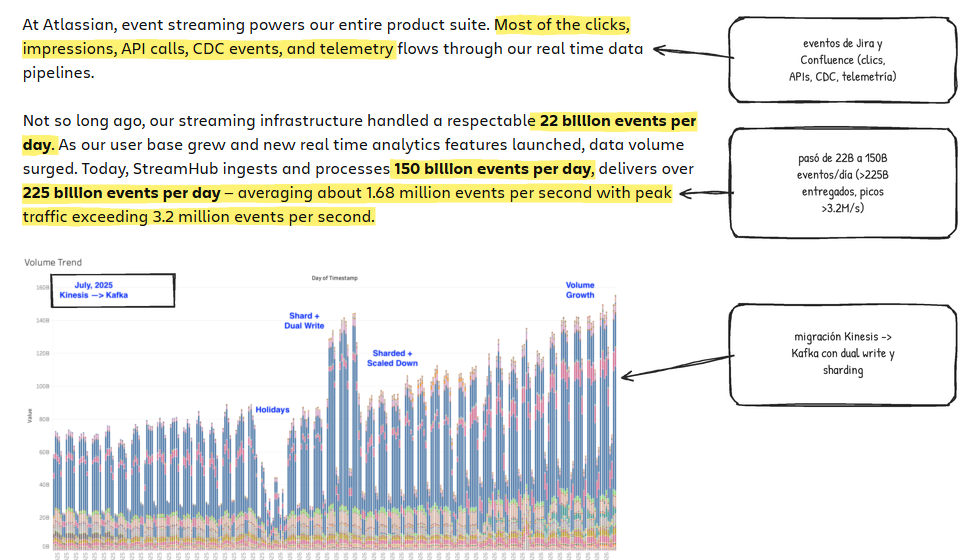
\includegraphics[width=0.92\textwidth]{capturas/fuente_streamhub_anotada.png}%
    }{%
        \fbox{\parbox{0.92\textwidth}{\centering\vspace{1.2cm}
        \textit{Archivo de imagen esperado: \texttt{capturas/fuente\_streamhub\_anotada.png}}
        \vspace{1.2cm}}}%
    }
    \caption{Fragmentos subrayados y anotados sobre la fuente técnica oficial del caso StreamHub en Atlassian \cite{kava2026streamhub}.}
\end{figure}

\subsection*{2. Sistema conocido de primera mano}

\subsection*{3. Declaración de uso de inteligencia artificial}

\newpage

% ==========================================================================
% Referencias bibliográficas (IEEE)
% ==========================================================================
\printbibliography[title={Referencias}]

\end{document}
